\section{Network Design Problem} \label{sec:7}

\subsection{The Framework of a Network Design Problem} \label{subsec:7.1}
Let $G = (V, E)$ be a 
graph with nonnegative costs $c_e \geq 0$ for all $e \in E$. 
Suppose we have some ``cut requirement'' function $f : 2^V \to \{0, 1\}$. 
The goal of the network design problem is to minimize 
\[ c(F) = \sum_{e \in F} c_e \] 
such that $F \subseteq E$ and $|F \cap \delta(S)| \geq 1$ for all $S 
\subseteq V$ satisfying $f(S) = 1$. 

We say that a function $f : 2^V \to \{0, 1\}$ is {\bf proper} if 
\begin{enumerate}[(i)]
    \item $f(V) = 0$;
    \item $f(V \setminus S) = f(S)$ for all $S \subseteq V$;
    \item $f(A \cup B) \leq \max\{f(A), f(B)\}$ for all nonempty
    subsets $A,B \subseteq V$ such that $A \cap B = \varnothing$. 
\end{enumerate}
Let's look at a few examples of network design problems with 
respect to proper cut requirement functions. 

{\bf Shortest $s,t$-paths.} Recall from CO 250 that the shortest $s,t$-path 
problem can be formulated as the IP 
\begin{align*}
    \min\quad & \sum_{e\in E} c_e x_e \\ 
    \text{subject to}\quad & \sum_{e\in \delta(S)} x_e \geq 1 
    \quad \text{for all $S \subseteq V$ such that $|S \cap \{s, t\}| = 1$} \\
    & x \geq \mathbf 0 \text{ and integer.}
\end{align*}
Here, we can assume that $x_e \in \{0, 1\}$ as this is a minimization problem,
and these values correspond to a choice of edges 
$F \subseteq E$. In particular, each constraint is equivalent to having 
$|F \cap \delta(S)| \geq 1$ for all $S \subseteq V$ with $|S \cap \{s, t\}| = 1$,
and the objective function is $c(F)$. Therefore, the shortest $s,t$-path can be 
modelled as a network design problem where the cut requirement function 
is given by 
\[ f(S) = \begin{cases}
    1 & \text{if } |S \cap \{s, t\}| = 1, \\ 
    0 & \text{otherwise.}
\end{cases} \] 
Let's check that this choice of $f : 2^V \to \{0, 1\}$ really is a proper function.
\begin{enumerate}[(i)]
    \item We have $f(V) = 0$ since $|V \cap \{s, t\}| = 2$. 
    \item This follows from the fact that if $s \in S$, then $s \notin V \setminus S$,
    and the same holds for $t$.
    \item Suppose towards a contradiction that there exist nonempty disjoint
    subsets $A, B \subseteq V$ such that $f(A \cup B) = 1$ and $f(A) = f(B) = 0$. 
    Then we have $|(A \cup B) \cap \{s, t\}| = 1$, which implies that 
    $A \cup B$ contains exactly one of $s$ or $t$. Without loss of generality, 
    suppose that $s \in A \cup B$ and $t \notin A \cup B$. Then we see that 
    $s$ must be in at least one of $A$ or $B$; without loss of generality, 
    suppose it is $A$. This implies that $s \in A$ and $t \notin A$, so 
    $f(A) = 1$, which is a contradiction.
\end{enumerate}

{\bf Minimum cost Steiner trees.} The minimum cost Steiner tree problem
with respect to some set of terminals $T \subseteq V$ 
can be viewed as a network design problem where the cut requirement 
function is given by 
\[ f(S) = \begin{cases}
    1 & \text{if $S \cap T \neq \varnothing$ and $S \cap T \neq T$}, \\
    0 & \text{otherwise.}
\end{cases} \] 
We check that this choice of $f : 2^V \to \{0, 1\}$ is proper. 
Conditions (i) and (ii) are clear, so we verify (iii). 

Suppose towards a contradiction that there are nonempty disjoint subsets $A, B \subseteq V$ 
such that $f(A \cup B) = 1$ and $f(A) = f(B) = 0$. This implies that 
$(A \cup B) \cap T \neq \varnothing$ and $(A \cup B) \cap T \neq T$. 
Since $A$ and $B$ are both subsets of $A \cup B$, it must be that 
$A \cap T \neq T$ and $B \cap T \neq T$. Moreover, since $(A \cup B) 
\cap T \neq \varnothing$, at least one of $A$ and $B$ must have 
nonempty intersection with $T$. Without loss of generality, we may assume 
that it is $A$. Then $A \cap T \neq \varnothing$ and $A \cap T \neq T$
so that $f(A) = 1$, which is a contradiction. 

{\bf Generalized minimum cost Steiner tree problem.} In this problem, 
we are given a graph $G = (V, E)$ and nonnegative costs $c_e \geq 0$ for all 
$e \in E$. Now, instead of just a single terminal $T \subseteq V$, 
we may be given multiple terminals $T_1, T_2, \dots, T_k \subseteq V$. Our 
goal is to minimize $c(F)$ over $F \subseteq E$, where for each $i = 1, \dots, k$, 
the vertices in $T_i$ are connected by the edges in $F$. 

For example, the graph below has three sets of terminals in blue, red, and green.
The bolded edges connect the vertices in all the terminals. We see that a 
subset which does this does not need to be connected itself, unlike the 
usual Steiner tree problem with one terminal.
\begin{center}
    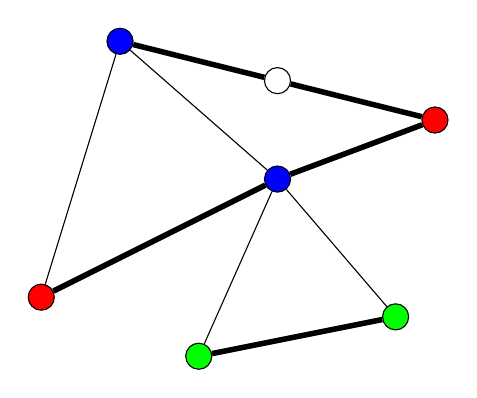
\begin{tikzpicture}[node distance={30mm}, main/.style = {draw, circle}] 
        \node[main, fill=blue] (1) at (4, 2) {}; 
        \node[main] (2) at (6, 1.5) {};
        \node[main, fill=red] (3) at (8, 1) {};
        \node[main, fill=blue] (4) at (6, 0.25) {};
        \node[main, fill=red] (5) at (3, -1.25) {};
        \node[main, fill=green] (6) at (5, -2) {};
        \node[main, fill=green] (7) at (7.5, -1.5) {};

        \draw [line width=2pt] (1) -- (2); \draw [line width=2pt] (2) -- (3);
        \draw [line width=2pt] (3) -- (4);
        \draw (1) -- (4); \draw (1) -- (5); 
        \draw [line width=2pt] (4) -- (5);
        \draw (4) -- (6); \draw (4) -- (7); \draw [line width=2pt] (6) -- (7);
    \end{tikzpicture} 
\end{center}\vspace{-0.25cm}
This problem can be formulated as a network design problem where the 
cut requirement function is
\[ f(S) = \begin{cases}
    1 & \text{if there exists $i = 1, \dots, k$ such that 
    $S \cap T_i \neq \varnothing$ and $S \cap T_i \neq T_i$}, \\
    0 & \text{otherwise.}
\end{cases} \] 
The fact that $f : 2^V \to \{0, 1\}$ is a proper function can be shown 
similarly to above.

\subsection{LP Formulation of the Network Design Problem} \label{subsec:7.2}
From now on, we assume that the cut requirement function 
$f : 2^V \to \{0, 1\}$ is proper. How do we solve network design problems 
under this assumption? This problem is $\NP$-hard in general 
since the Steiner tree problem is a special case of it. 
But we have nice approximation algorithms by way of linear programming. 

First, for ease of notation, we'll denote $\mathcal{K} = \{S \subseteq V : 
f(S) = 1\}$. Then the LP formulation of the network design problem, 
namely our primal LP (P), can be stated as follows. 
\begin{align*}
    \min\quad & \sum_{e\in E} c_e x_e \\ 
    \text{subject to}\quad & \sum_{e\in \delta(S)} x_e \geq 1 
    \quad \text{for all $S \in \mathcal{K}$} \\
    & x \geq \mathbf 0.
\end{align*}
Then the dual LP of (P), say (D), is given as follows.
\begin{align*}
    \max\quad & \sum_{S\in\mathcal{K}} 1 \cdot y_S \\ 
    \text{subject to}\quad & \sum_{S\in\mathcal{K}\,:\,e \in \delta(S)} y_S \leq c_e 
    \quad \text{for all $e\in E$} \\
    & y \geq \mathbf 0.
\end{align*}

\subsection{Iterative Rounding Approach} \label{subsec:7.3}
The iterative rounding approach for solving network design problems 
only makes use of the primal LP (P) above. The algorithm is
as follows: 
\begin{mdframed}[
    linewidth=1pt,
    linecolor=black,
    bottomline=false,topline=false,rightline=false,
    innerrightmargin=0pt,innertopmargin=0pt,innerbottommargin=0pt,
    innerleftmargin=1em,% Distance between vertical rule & proof content
    skipabove=0.75\baselineskip
]
{\bf Input.} A graph $G = (V, E)$, edge costs $c_e \geq 0$ for 
all $e \in E$, and a cut requirement function $f : 2^V \to \{0, 1\}$. 

{\bf Output.} A set of edges $F \subseteq E$ with value close to the optimum.
\begin{enumerate}[leftmargin=1.75cm, label={Step \arabic*.}]
    \item [{Step 0.}] Initialize $F \gets \varnothing$.
    \item Find an extreme optimal solution $\bar{x}$ for the primal LP
    (which can be done in polynomial time).

    \item Find $e' \in E$ such that $\bar{x}_{e'} = 0$ or $\bar{x}_{e'} \geq 1/2$.
    The existence of such an edge for $\bar{x}$ is guaranteed to 
    exist in the case where $f : 2^V \to \{0, 1\}$ is a proper function.

    \item If $\bar{x}_{e'} = 0$, then construct $G' = (V, E \setminus \{e\})$
    and keep the same costs for the remaining edges. 
    If $\bar{x}_{e'} \geq 1/2$, construct $G'$ from $G$ by contracting the 
    edge $e'$ and include $e'$ into $F$. 

    \item Recursively call the algorithm on $G'$ to obtain a solution $F'$. 
    Output $F \gets F' \cup F$. 
\end{enumerate}
\end{mdframed}\vspace{-0.25cm}
Note that the optimal value $\text{OPT}_{\text{primal IP}}$ for the network 
design problem is the optimal value of the primal LP (P) with added 
integrality constraints. By solving the primal LP, we only obtain 
the value $\text{OPT}_{\text{primal LP}}$, which gives us a lower
bound on the desired value via
\[ \text{OPT}_{\text{primal LP}} \leq \text{OPT}_{\text{primal IP}} \] 
since this is a minimization problem and any feasible solution to the IP is 
also feasible for the LP. It turns out that the iterative rounding 
approach produces a solution of cost at most $2 \cdot \text{OPT}_{\text{primal LP}}$
and hence at most $2 \cdot \text{OPT}_{\text{primal IP}}$. In particular, 
the iterative rounding approach is a $2$-approximation algorithm for the 
network design problem.

We won't prove that an edge $e' \in E$ such that $\bar{x}_{e'} = 0$ 
or $\bar{x}_{e'} \geq 1/2$ always exists when $f : 2^V \to \{0, 1\}$ is a 
proper function, as this is quite difficult. For the analysis, we'll assume 
this fact and show that the solution obtained of the algorithm is within a 
factor of $2$ of the optimum. This can be proven by induction on the number 
of edges $|E|$. 

{\bf Case 1.} Suppose that $\bar{x}_{e'} = 0$. Then the solution 
$x^*_e := \bar{x}_e$ for all $e \in E \setminus \{e'\}$ is still feasible 
for the LP constructed for $G' = (V, E \setminus \{e'\})$. By 
induction, we have that 
\[ c(F') \leq 2 \cdot \text{OPT}_{\text{primal LP for $G'$}} \leq 
2 \cdot \sum_{e \in E} c_e \bar{x}_e \leq 2 \cdot \text{OPT}_{\text{primal LP}}, \] 
where $F'$ is the output of the algorithm for $G'$.

{\bf Case 2.} Suppose that $\bar{x}_{e'} \geq 1/2$. Then the solution 
$x_e^* := \bar{x}_e$ for all $e \in E \setminus \{e'\}$ is still feasible 
for the LP constructed for $G'$ obtained by contracting $e'$ in $G$. 
By induction, we have that 
\[ c(F') \leq 2 \cdot \text{OPT}_{\text{primal LP for $G'$}} \leq 
2 \cdot \sum_{e \in E \setminus \{e'\}} c_e \bar{x}_e, \]
where $F'$ is the output of the algorithm for $G'$. Afterwards, we output 
$F' \cup \{e'\}$ for $G$, and we see that 
\[ c(F' \cup \{e'\}) \leq 2 \cdot \sum_{e \in E \setminus \{e'\}} c_e \bar{x}_E
+ c'_e \leq 2 \cdot \sum_{e \in E} c_e \bar{x}_e \] 
since $c_{e'} \leq 2c_{e'} \bar{x}_{e'}$ by the choice of $e'$, as desired. 

\subsection{Primal-Dual Approach} \label{subsec:7.4}
We now give another approximation algorithm for solving the network 
design problem, this time making use of the dual LP. The idea is to 
construct a feasible solution $y$ for the dual LP; based on this 
dual solution $y$, we construct the output $F \subseteq E$. Suppose we 
could argue that 
\[ c(F) \leq \alpha \cdot \sum_{S \in \mathcal{K}} y_S \] 
where $\sum_{S \in \mathcal{K}} y_S$ is the value of the dual solution $y$ 
and $\alpha \geq 1$ is some constant. We see that 
\[ \sum_{S\in\mathcal{K}} y_S \leq \text{OPT}_{\text{primal LP}} \leq 
\text{OPT}_{\text{primal IP}} \] 
where the first inequality is due to weak duality. This gives rise to an
$\alpha$-approximation algorithm.

The primal-dual approach is based on the notion of continuous growth. 
Over a time period, we pick some values $y_S$ where $S \in \mathcal{K}$
and increase them at the same rate, while the other values are kept fixed. 
\begin{enumerate}[(1)]
    \item At a time period, how do we select the subsets $S \in \mathcal{K}$ 
    for which to increase the values $y_S$?
    \item When do we stop increasing the values for the currently 
    selected sets $S \in \mathcal{K}$?
\end{enumerate}
To answer the first question, we will pick all the inclusion-wise minimal sets 
$S \in {\cal K}$ such that $\delta(S) \cap F = \varnothing$. In other words, 
these are the sets $S \subseteq V$ such that $f(S) = 1$ and $\delta(S) \cap F 
= \varnothing$, with the property that any proper subset $S' \subsetneq S$ will have 
$f(S') = 0$ or $\delta(S') \cap F \neq \varnothing$. 

Let $\mathcal{B} := \{S \in \mathcal{K} : \delta(S) \cap F = \varnothing\}$. 
We call $\mathcal{B}$ the collection of violated sets. Let
$\mathcal{D}$ be the collection of minimal sets in $\mathcal{B}$. The following 
lemma tells us that $\mathcal{D}$ can be efficiently computed.

\begin{lemma}{lemma:7.1} 
    For every $F \subseteq E$, we have that 
    \[ \mathcal{D} = \{S \subseteq V : \text{$S$ is a connected component of $(V, F)$ 
    such that $f(S) = 1$}\}. \]
\end{lemma}\vspace{-0.25cm}
\begin{pf}[Lemma~\ref{lemma:7.1}]
    $(\subseteq)$  Let $S_1, \dots, S_k$ denote the connected components of $(V, F)$, 
    and let $S \subseteq V$. If $S \cap S_i \neq \varnothing$ and 
    $S \cap S_i \neq S_i$, then we have $F \cap \delta(S) \neq \varnothing$. 
    In particular, for any $S \in \mathcal{B}$, we have that 
    \[ S = \bigcup_{j \in J} S_j \] 
    for some $J \subseteq \{1, \dots, k\}$. Since $f : 2^V \to \{0, 1\}$ 
    is a proper function, we have 
    \[ f(S) \leq \max_{j\in J} f(S_j). \] 
    Let $S \in \mathcal{D}$ so that $S$ is a minimal set in $\mathcal{B}$.
    By the above discussion, we can write $S = \bigcup_{j\in J} S_j$ for 
    some $J \subseteq \{1, \dots, k\}$. Since $f(S) = 1$, we see that 
    $f(S_j) = 1$ for some $j \in J$. Then $S_j$ is a connected component 
    of $(V, F)$, which implies that $\delta(S_j) \cap F = \varnothing$. 
    Therefore, $S_j$ is a violated set. Since $S$ is minimal, 
    it must be that $S = S_j$ for some $j = 1, \dots, k$, so $S$ 
    is a connected component of $(V, F)$. 

    $(\supseteq)$ Suppose that $S$ is a connected component of $(V, F)$. 
    Then $\delta(S) \cap F = \varnothing$, so $S$ is a violated set. 
    But for every nonempty proper subset $S' \subsetneq S$, we have 
    $\delta(S') \cap F \neq \varnothing$ because inside the connected 
    component, considering the cut induced by some proper subset of vertices 
    gives rise to an edge. This implies that $S$ must be minimal, so 
    we are done. \qed 
\end{pf}\vspace{-0.25cm}

As a consequence, we obtain the following corollary. 

\begin{cor}{cor:7.2}
    A subset $F \subseteq E$ is a feasible solution to the network design 
    problem if and only if for every component $S$ of $(V, F)$, 
    we have $f(S) = 0$. 
\end{cor}\vspace{-0.25cm}

Now, let's consider the question of when to stop increasing the values of $y_S$. 
As stated before, we will increase the values of $y_S$ for all $S \in \mathcal{D}$
at the same rate, and leave $y_S$ for $S \notin \mathcal{D}$ unchanged. 
We do this until there is an edge $e \in E$ such that $e \in \delta(S)$ 
for some $S \in \mathcal{D}$ and 
\[ \sum_{S\in\mathcal{K}\,:\,e\in\delta(S)} y_S = c_e. \] 
That is, the corresponding constraint for $e \in E$ in the dual LP becomes tight. 
In this case, we call the edge $e$ {\bf tight}. Once we stop, we will 
include all the tight edges into $F$. 

Putting everything together, the primal-dual approach to solve network 
design problems is as follows.

\begin{mdframed}[
    linewidth=1pt,
    linecolor=black,
    bottomline=false,topline=false,rightline=false,
    innerrightmargin=0pt,innertopmargin=0pt,innerbottommargin=0pt,
    innerleftmargin=1em,% Distance between vertical rule & proof content
    skipabove=0.75\baselineskip
]
{\bf Input.} A graph $G = (V, E)$, edge costs $c_e \geq 0$ for 
all $e \in E$, and a cut requirement function $f : 2^V \to \{0, 1\}$. 

{\bf Output.} A set of edges $F \subseteq E$ with value close to the optimum.
\begin{enumerate}[leftmargin=1.75cm, label={Step \arabic*.}]
    \item Let $F = \varnothing$ and let $y_S = 0$ for all $S \in \mathcal{K}$.
    Let $\mathcal{D}$ be the collection of minimal violated sets with respect 
    to $F$. (At this stage, these are the sets of isolated vertices in ${\cal K}$.)

    \item While $\mathcal{D} \neq \varnothing$:
    \begin{enumerate}[label={Step 2.\arabic*.}]
        \item Increase $y_S$ for $S \in \mathcal{D}$ at the same rate 
        until some edge $e \in E$ becomes tight.
        \item Update $F := F \cup T$ where $T$ is the set of all tight edges. 
        Update $\mathcal{D}$ with respect to this new $F$. 
    \end{enumerate}

    \item {\bf (Reverse delete.)} Let $F = \{e_1, \dots, e_k\}$ where the 
    index corresponds to the order that the edges were inserted to $F$. 
    Iterate backwards through the list; that is, start from $i = k$ 
    and go down to $i = 1$. For each $i$, if $F \setminus \{e_i\}$ is feasible 
    for the network design problem, update $F := F \setminus \{e_i\}$.
\end{enumerate}
\end{mdframed}\vspace{-0.25cm}
Let's look at an example of applying the primal-dual algorithm. 

{\bf Shortest $s,t$-paths.} Recall that this problem can be modelled 
as a network design problem with the proper cut requirement function 
$f : 2^V \to \{0, 1\}$ defined by 
\[ f(S) = \begin{cases}
    1 & \text{if } |S \cap \{s, t\}| = 1, \\ 
    0 & \text{otherwise.}
\end{cases} \] 
Consider the following graph $G = (V, E)$, where we want to find the shortest 
path from $s$ to $t$.
\begin{center}
    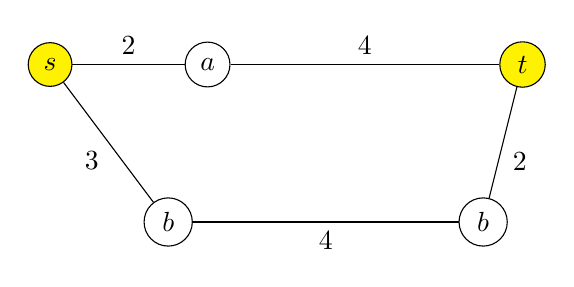
\begin{tikzpicture}[node distance={30mm}, main/.style = {draw, circle}] 
        \node[main, fill=yellow] (s) at (0, 0) {$s$}; 
        \node[main] (a) at (2, 0) {$a$};
        \node[main, fill=yellow] (t) at (6, 0) {$t$};
        \node[main] (b) at (1.5, -2) {$b$};
        \node[main] (c) at (5.5, -2) {$b$};

        \draw (s) -- (a) node[midway, above] {2};
        \draw (s) -- (b) node[midway, below left] {3};
        \draw (a) -- (t) node[midway, above] {4};
        \draw (b) -- (c) node[midway, below] {4};
        \draw (c) -- (t) node[midway, below right] {2};
    \end{tikzpicture} 
\end{center}\vspace{-0.25cm}
At Step 1, we initialize $F = \varnothing$ and $y_S = 0$ for all $S \in {\cal K}$. 
The collection of minimal violated sets with respect to $F = \varnothing$ is 
${\cal D} = \{\{s\}, \{t\}\}$, because at this point, every set $S \in {\cal K}$ 
is violated, and these are the minimal sets containing exactly one of $s$ or $t$.

Next, we enter the while loop. We grow the $y_S$ values for $S \in {\cal D}$ 
uniformly until an edge becomes tight. This happens when $y_{\{s\}} = y_{\{t\}} = 2$, 
where both the edges $sa$ and $ct$ become tight. We update 
$F = \{sa, ct\}$, and the collection of minimal violated sets with respect to 
$F = \{sa, ct\}$ is ${\cal D} = \{\{s, a\}, \{c, t\}\}$.

\begin{center}
    \begin{tikzpicture}[node distance={30mm}, main/.style = {draw, circle}] 
        \node[main, fill=yellow] (s) at (0, 0) {$s$}; 
        \node[main] (a) at (2, 0) {$a$};
        \node[main, fill=yellow] (t) at (6, 0) {$t$};
        \node[main] (b) at (1.5, -2) {$b$};
        \node[main] (c) at (5.5, -2) {$c$};
        \node[draw, color=red, inner sep=0pt, circle, yscale=0.95, fit={(s)}] {};
        \node[draw, color=red, inner sep=0pt, circle, yscale=0.95, fit={(t)}] {};
        \node[color=red] (iter1s) at (-0.5, 0.25) {\small $2$};
        \node[color=red] (iter1t) at (6.5, 0.25) {\small $2$};

        \draw [color=red] (s) -- (a) node[midway, above] {2};
        \draw (s) -- (b) node[midway, below left] {3};
        \draw (a) -- (t) node[midway, above] {4};
        \draw (b) -- (c) node[midway, below] {4};
        \draw [color=red] (c) -- (t) node[midway, below right] {2};
    \end{tikzpicture} 
\end{center}\vspace{-0.25cm}

During the next iteration, we increase the $y_S$ values for $S \in {\cal D}$ 
again until another edge becomes tight. This happens when $y_{\{s, a\}} 
= y_{\{c, t\}} = 1$, in which case edges $sb$ and $at$ become tight since 
$y_{\{s\}} + y_{\{s, a\}} = 2 + 1 = 3 = c_{sb}$ and 
$y_{\{t\}} + y_{\{s,a\}} + y_{\{c,t\}} = 2 + 1 + 1 = 4 = c_{at}$.
We update $F = \{sa, ct, sb, at\}$. There are no more violated 
sets, so we exit the while loop since ${\cal D} = \varnothing$. 

\begin{center}
    \begin{tikzpicture}[node distance={30mm}, main/.style = {draw, circle}] 
        \node[main, fill=yellow] (s) at (0, 0) {$s$}; 
        \node[main] (a) at (2, 0) {$a$};
        \node[main, fill=yellow] (t) at (6, 0) {$t$};
        \node[main] (b) at (1.5, -2) {$b$};
        \node[main] (c) at (5.5, -2) {$c$};
        \node[draw, color=red, inner sep=0pt, circle, yscale=0.95, fit={(s)}] (iter1sc) {};
        \node[draw, color=red, inner sep=0pt, circle, yscale=0.95, fit={(t)}] (iter1tc) {};
        \node[color=red] (iter1s) at (-0.5, 0.25) {\small $2$};
        \node[color=red] (iter1t) at (6.5, 0.25) {\small $2$};
        \node[draw, color=blue, inner sep=0pt, ellipse, yscale=1, fit={(s) (a) (iter1sc) (iter1s)}] {};
        \node[draw, color=blue, inner sep=0pt, ellipse, yscale=1, fit={(t) (c) (iter1tc) (iter1t)}] {};
        \node[color=blue] (iter2s) at (-0.5, 0.75) {\small $1$};
        \node[color=blue] (iter2t) at (7, 0.25) {\small $1$};

        \draw [color=red] (s) -- (a) node[midway, above] {2};
        \draw [color=blue] (s) -- (b) node[midway, below left] {3};
        \draw [color=blue] (a) -- (t) node[midway, above] {4};
        \draw (b) -- (c) node[midway, below] {4};
        \draw [color=red] (c) -- (t) node[midway, below right] {2};
    \end{tikzpicture} 
\end{center}\vspace{-0.25cm}

Now, we go to the reverse delete step. We initially have $F = \{sa, ct, sb, at\}$. 
Going backwards, we see that $at$ cannot be removed as $F \setminus \{at\}$ 
is no longer feasible for the shortest $s,t$-path problem. Next, we 
see that $sb$ can be removed and so can $ct$, so our final result is 
$F = \{sa, at\}$. 

\subsection{Efficiency of the Primal-Dual Algorithm} \label{subsec:7.5}
In order to implement the primal-dual algorithm efficiently, we will 
only keep track of the nonzero values $y_S$ for $S \in {\cal K}$. 
There are up to $2^{|V|}$ entries in $y$, so it will be extremely 
inefficient to set all of them to $0$ at the start of the algorithm.
We only need $y$ to keep track of tightness; that is, whether or not
$c_e = \sum_{S \in {\cal K}\,:\,e \in \delta(S)} y_S$. 

The computation of ${\cal D}$ in each iteration of Step 2 
can be done efficiently using Lemma~\ref{lemma:7.1}, which states that 
\[ \mathcal{D} = \{S \subseteq V : \text{$S$ is a connected component of $(V, F)$ 
such that $f(S) = 1$}\}. \]
Note that $(V, F)$ has exactly $|V|$ components at the start of the 
algorithm, and in each iteration of Step 2, the number of connected 
components of $(V, F)$ decreases. Hence, there are at most 
$|V|$ iterations of Step 2. Moreover, we have that $|{\cal D}| \leq |V|$, 
so during each iteration, at most $|V|$ of the $y_S$ values become nonzero.
Therefore, at the end of the algorithm, there are at most $|V| \times |V| = 
|V|^2$ nonzero $y_S$ values for $S \in {\cal K}$. 

We cannot actually implement continuous growth, so we need a different 
way of doing so. Instead, the $y_S$ values will be increased by 
\[ \min_{e\in E} \left\{ \frac{1}{|\{S \in {\cal D} : e \in \delta(S)\}|} 
\left( c_e - \sum_{S \in {\cal K}\,:\,e \in \delta(S)} y_S \right) \right\} \] 
at once, and this value can be efficiently computed.

Finally, reverse delete can be implemented efficiently by computing 
${\cal D}$ with respect to $F \setminus \{e_i\}$ for each edge $e_i$ 
and checking whether or not ${\cal D}$ is empty.

\subsection{Approximation Guarantee of the Primal-Dual Algorithm} \label{subsec:7.6}
Let $F \subseteq E$ be the set of edges returned by the primal-dual algorithm, 
and let $y$ be the solution to the dual LP at the end of the algorithm. 
We will show that 
\[ \sum_{e \in F} c_e \leq 2 \sum_{S \in {\cal K}} y_S, \] 
Assuming this, we obtain 
\[ \sum_{e \in F} c_e \leq 2 \sum_{S \in {\cal K}} y_S \leq 2 \cdot 
\text{OPT}_{\text{dual LP}} = 2 \cdot \text{OPT}_{\text{primal LP}} 
\leq 2 \cdot \text{OPT}_{\text{primal IP}}. \] 
Note that if $e \in F$, then we are guaranteed that $e$ is tight, so 
\[ c_e = \sum_{S \in {\cal K}\,:\,e \in \delta(S)} y_S. \]
This gives us one part of complementary slackness. However, it does not 
need to be true in general that for every $S \in {\cal K}$ with 
$y_S > 0$, we have $|F \cap \delta(S)| = 1$. It might not even be true that 
for every $S \in {\cal K}$ with $y_S > 0$, we have $|F \cap \delta(S)| \leq 2$,
which would immediately imply that $\sum_{e \in F} c_e \leq 2 \sum_{S \in {\cal K}} y_S$.

Let's fix some notation. Let $t$ be the number of iterations of Step 2. 
For each $i = 1, \dots, t$:
\begin{itemize}
    \item Let ${\cal D}_i$ be the collection of minimal violated sets 
    at the beginning of the $i$-th iteration of Step 2.
    \item Let $\Delta_i$ be the ``duration'' of the $i$-th iteration of 
    Step 2. That is, $\Delta_i$ is equal to how much we increased 
    the $y_S$ values for $S \in {\cal D}_i$, while others stay fixed. 
    \item Let $F_i \subseteq E$ be the set of edges in $F$ at the 
    start of the $i$-th iteration of Step 2.
\end{itemize}

\begin{lemma}{lemma:7.3}
    For every $i = 1, \dots, t$, we have that
    \[ \sum_{S \in {\cal D}_i} |F \cap \delta(S)| \leq 2|{\cal D}_i|. \] 
\end{lemma}\vspace{-0.25cm}

Before we prove the lemma, let's see how this implies the desired inequality. 

\begin{theo}{theo:7.4}
    We have the inequality
    \[ \sum_{e \in F} c_e \leq 2 \sum_{S \in {\cal K}} y_S. \] 
    In particular, the primal-dual algorithm is a $2$-approximation algorithm 
    for the network design problem. 
\end{theo}\vspace{-0.25cm}
\begin{pf}[Theorem~\ref{theo:7.4}]
    Since $y_S$ increases by $\Delta_i$ at iteration $i$ whenever $S$ 
    is a minimal violated set for every $S \in {\cal K}$, we have 
    \[ y_S = \sum_{i=1,\dots, t\,:\,S \in {\cal D}_i} \Delta_i. \] 
    Then we obtain 
    \begin{align*}
        c(F) = \sum_{e \in F} c_e 
        &= \sum_{e \in F} \sum_{S \in {\cal K}\,:\,e\in\delta(S)} y_S \\
        &= \sum_{S \in {\cal K}} |\delta(S) \cap F| y_S \\ 
        &= \sum_{S \in {\cal K}} |\delta(S) \cap F| \sum_{i=1,\dots, t\,:\,S \in {\cal D}_i} \Delta_i \\ 
        &= \sum_{i=1}^t \Delta_i \sum_{S \in {\cal D}_i} |\delta(S) \cap F| \\ 
        &\leq \sum_{i=1}^t \Delta_i \cdot 2|{\cal D}_i| \\ 
        &= 2 \sum_{S \in {\cal K}} \sum_{i=1,\dots, t\,:\,S \in {\cal D}_i} \Delta_i \\ 
        &= 2 \sum_{S \in {\cal K}} y_S,
    \end{align*}
    where the inequality follows from Lemma~\ref{lemma:7.3}. \qed 
\end{pf}\vspace{-0.15cm}

We now prove the lemma, which did the bulk of the work in giving us the 
approximation guarantee. 

\begin{pf}[Lemma~\ref{lemma:7.3}]
    Let $G' = (U, H)$ be the graph obtained from the original graph 
    $G = (V, E)$ after contracting the connected components of $(V, F_i)$ 
    independently. For each $u \in U$, let $S_u \subseteq V$ denote the 
    vertices of $G$ that were contracted to obtain $u$ in $G'$. 
    Note that $H$ has no edges in $F_i$ as they have been contracted, 
    but $H$ may contain parallel edges. Proving the lemma is now equivalent 
    to showing that 
    \[ \sum_{u\in U\,:\,S_u \in {\cal D}_i} |\delta(S_u) \cap F| \leq 
    2 \cdot |\{u\in U : S_u \in {\cal D}_i\}|. \] 
    {\bf Claim 1.} $(U, F \cap H)$ does not contain any cycles. 

    {\bf Proof of Claim 1.} Suppose by way of contradiction that 
    $(U, F \cap H)$ contains some cycle $C'$. Let $g$ be the last 
    edge from $C'$ that was added to $F$. We consider the point 
    in time when $g$ was considered during the reverse delete step. 
    Note that $g$ is contained in some cycle $C$ formed by some 
    of the edges in $C' \cup F_i$. When $g$ is considered during 
    reverse delete, all the edges in $C$ are still present. 
    It follows that $g$ is removed during reverse delete, contradicting 
    the fact that $g$ is part of the final output $F$ of the algorithm. 
    \hfill $\blacksquare$

    {\bf Claim 2.} For every $u \in U$ such that $S_u \notin {\cal K}$, 
    we have $|\delta(S_u) \cap F| \geq 2$ or $|\delta(S_u) \cap F| = 0$. 
    In particular, for every $u \in U$ with $S_u \notin {\cal D}_i$,
    we have $|\delta(S_u) \cap F| \geq 2$ or $|\delta(S_u) \cap F| = 0$.

    {\bf Proof of Claim 2.} Assume that there is some $u \in U$ 
    with $S_u \notin {\cal K}$ such that $|\delta(S_u) \cap F| = 1$. 
    Let $g$ be the edge in $\delta(S_u) \cap F$. Since $g$ was not 
    removed during reverse delete, there is some $S \subseteq U$ 
    such that $\delta(\bigcup_{v\in S} S_v) \cap F = \{g\}$ 
    and $\bigcup_{v\in S} S_v \in {\cal K}$. 
    
    Let $C_1, \dots, C_k \subseteq U$ denote the connected components 
    of $(U, F \cap H)$. Since $\delta(\bigcup_{v\in S} S_v) \cap F = \{g\}$, 
    we see for every connected component $C_i$ such that 
    $u \notin C_i$, we have $C_i \subseteq S$ or $C_i \cap S = \varnothing$. 
    Then without loss of generality, we may write 
    $S = \{u\} \cup \bigcup_{j \in J} C_j$
    where $J \subseteq \{1, \dots, k\}$ and $u \notin C_j$ for all $j \in J$. 
    Since $C_j$ are connected components of $(U, F \cap H)$ and 
    $F$ is a feasible solution for the network design problem, we have 
    $\bigcup_{v \in C_j} S_v \notin {\cal K}$ for all $j = 1, \dots, k$. 
    Moreover, we have $S_u \notin {\cal K}$ by assumption. But then 
    \[ \bigcup_{v \in S} S_v = S_u \cup \bigcup_{j \in J} \bigcup_{v \in C_j} S_v \notin {\cal K} \] 
    since the cut requirement function $f : 2^V \to \{0, 1\}$ is proper. 
    This is a contradiction. \hfill $\blacksquare$
    
    We'll call the connected components consisting of only vertex trivial 
    as they have no edges. Combining the claims, we have that 
    \begin{align*}
        \sum_{u\in U\,:\,S_u\in {\cal D}_i} |\delta(S_u) \cap F| 
        &= \sum_C \sum_{u\in C\,:\,S_u \in {\cal D}_i} |\delta(S_u) \cap F| \\ 
        &= \sum_C \left( \sum_{u\in C} |\delta(S_u) \cap F| - \sum_{u\in C\,:\,S_u \notin {\cal D}_i} |\delta(S_u) \cap F| \right) \\ 
        &\leq \sum_C \left( 2(|C| - 1) - \sum_{u\in C\,:\,S_u \notin {\cal D}_i} 2 \right) \\ 
        &\leq 2 \cdot \sum_C (|C| - |\{u \in C : S_u \notin {\cal D}_i\}|) \\ 
        &= 2 \cdot \sum_C |\{u \in C: S_u \in {\cal D_i}\}| \leq 2 \cdot |\{u \in U : S_u \in {\cal D}_i\}|, 
    \end{align*}
    where the sums over $C$ above range over the nontrivial connected components $C$ of 
    $(U, F \cap H)$. We use both Claim 1 and Claim 2 in the first inequality. 
    Claim 1 guarantees that in a connected component $C$ of $(U, F \cap H)$, 
    the edges of $F$ form a tree. This means that $F$ has exactly 
    $|C| - 1$ edges with at least one of the endpoints in $C$. \qed 
\end{pf}